\section{Movie Subtitles}
\subsection{Subtitles in General}

Subtitles are textual versions of the dialog in films or television shows which are shown on the screen at the same time the dialogs are performed. The most common reasons to show the subtitles is either to allow the deaf of hard-of-hearing viewers to follow the dialogs or to allow viewers who are not speakers of the language used in the movie to understand the movie while hearing the original sound track. The major difference between these two types of subtitling is that the subtitles for deaf people usually contains not only the dialogs, but also a lot additional information, e.g. that music is playing or description of other noises important for the story. 

Originally, the subtitles used to be chemically corroded or leaser burnt into the film tape. While using the digital technology, the subtitles can be added dynamically to the screen and do not have to be actual part of the movie. Moreover, they can be distributed independently on the movie. The subtitles are in a standalone file which contains the subtitles and some meta data telling the players which subtitle chunks should be displayed at the which time interval.

While making a professional translation of the subtitles, the translator have the whole screenplay of the movie, accompanied with a lot of notes concerning the expressiveness of the utterances and using the rhetorical devices (culture references, sarcasm etc.), on the other hand the often do not see the movie. They are equipped with the same tools as other professional translators as translation memories or glossaries checking the consistence of used vocabulary.

On the other hand, the fan translators use simple editors without any special functionality and usually watch the movie during translating.

Some info, how should the subtitles look like here: 
http://www.ofcom.org.uk/static/archive/itc/itc_publications/codes_guidance/standards_for_subtitling/subtitling_1.asp.html
(maybe add a summary of that)

\subsection{Subtitle Formats}
\label{subtitle_formats}

There is a lot of subtitle formats, most of them proprietary. The most widely is the SubRip srt format. Sometimes also MicroDVD sub format is used. Example of the formats is in table \ref{subtitleFormats}.

\begin{table}
\begin{center}
\begin{tabular}{cc}
\fbox{\parbox{7.5cm}{\tt4\\
00:02:04,718 --$>$ 00:02:08,054\\
I just want to be alone with her\\
and hold her and kiss her\\
\\
5\\
00:02:08,179 --$>$ 00:02:12,309\\
and tell her how much l love her\\
and take care of her.\\
}} & \fbox{\parbox{7.5cm}{\tt
\{1025\}\{1110\}I just want to be alone with her|and hold her and kiss her\\

\{1375\}\{1460\}and tell her how much l love her|and take care of her.
}}
\end{tabular}
\end{center}

\caption{An example of the subtitle file formats, \emph{srt} at the left, \emph{sub} at the right side.}
\label{subtitleFormats}
\end{table}

The \emph{srt} file does not have any header and contains everything as text. Each subtitle chunk contains three or four lines and is separated from the previous and the next one by an empty line. The first line is the order of the subtitle in the movie, the second line contains the absolute time in the movie when the subtitle shows up and when it disappears. The time is expressed with the precision of thousandths of seconds. On the next one or two lines is the actual text of the subtitle. Standardly it should not contain any formating data, but the players usually support simple HTML-like formating tags.

In the MicroDVD sub format each line represents a subtitle. Numbers of frames in the video between whose the subtitle is displayed are used instead of absolute time. After the frame numbers in brackets, the actual text of the subtitle follows. The pipe symbol is used the line separator. The are also other proprietary format having the extension .sub, but they look differently.


\subsection{Current tools}

There are several freeware tools for amateur subtitle translation. They are usually standalone applications. The GUI of such applications typically consists of two columns, the first one with the subtitle chunks in the original language, the second one to be complete with the translation. Some of them offer also the synchronized playback of video during the translation. We did not find an application which would be web based and specialized on for the subtitles translation. An overview of such tool is in table \ref{subtitles_tools}

\begin{table}[h]

\begin{center}
\begin{tabular}{|c|c|c|c|}
\hline
\bf name & \bf licence & \bf platform & \bf website \\
\hline
Subtitle Workshop 4 & freeware & Windows & www.urusoft.net \\
\hline
Subtitle Processor & GPL & Windows & sourceforge.net/projects/subtitleproc \\
\hline
Open Subtitle Translator & GPL & Windows / Linux & sourceforge.net/projects/opensub \\
\hline
Gnome Subtitles & GPL & Linux & sourceforge.net/projects/gnome-subtitles \\
\hline
Subtitles Translator & freeware & Windows & www.mironto.sk \\ \hline

\end{tabular}
\end{center}

\caption{An overview of subtitle translation tools available on the Internet.} \label{subtitles_tools}
\end{table}

From our view there is also an interesting project by Google -- Google Translator Toolkit. It is a web application designed to help the translators with their work which also supports parsing subtitles. During his work, a translator can see the document both in source and target language and is given per sentence suggestions from the Google Translate or his own translation memory which the user has previously imported. When the work is finished created translation can be exported as a translation memory. This tool did not became popular among the translator, probably because of the quality of the machine translation provided. Professional translator would be also aware to bring their valuable translation memories to Google for free. 

\begin{figure}

\begin{center}
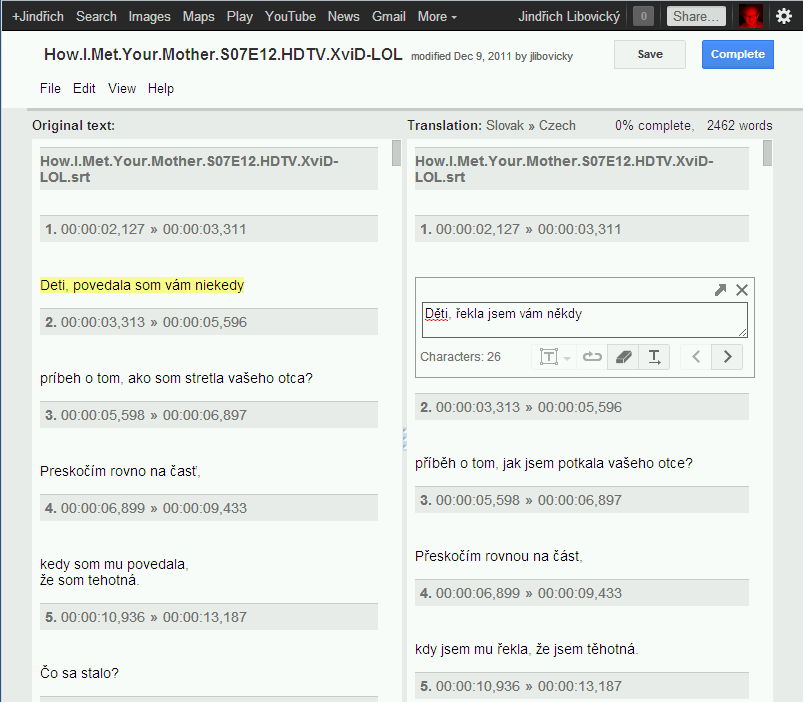
\includegraphics[scale=0.4]{./figures/google_translator_toolkit.png}
\end{center}

\caption{Google Translator Toolkit} \label{google_translator_toolkit}
\end{figure}

\section{Translation Memories}
\subsection{What is a Translation Memory}

A \emph{translation memory} is a tool for a computer assisted human translation. The core idea behind translation memories is the assumption that sentences that are similar in the source language will probably have a similar translation in the target language. Then, if the tool is able to provide the translator a translation of a similar sentence, there is a big chance the translator can just edit a little the provided sentence and get the translation he wants.

The translation memories are widely used in the translation industry, mostly while translating technical documentation and localization of software. In such cases the translators usually take advantage from that the new version of manuals of software does not differ much from the previous version. A survey \footnote{Elina Lagoudaki (2006), "Translation Memory systems: Enlightening users' perspective. Key finding of the TM Survey 2006 carried out during July and August 2006. (Imperial College London, Translation Memories Survey 2006), p.16} among companies producing multilingual documentation for their products in 2006 showed that 82.5 \% out of 874 such companies uses a TM system.

While using a translation memory there is usually an tendency to keep the database as clean as possible in terms of domain -- to contain only relevant for translated topics. The reasons to do so are the effort to keep the database as small as possible in order to not make the database search too slow and not spoil the terminology that is used in the particular area. To keep the the terminology consistent the domain glossaries are usually used.

There are several reasons why using translation memories makes the translators' work more efficient. The main advantage is that it reduces the cost and makes the translation process faster because the amount of the translators work is lower -- the work that has been done once can be easily reused. It helps to keep consistency of translation between more documents and also with their previous versions. It is also quite easy to ensure that each sentence of the original document was translated into a segment of the target language document.

There also some obstacles in using the translation memory systems. The professional Translation Memory Management Systems are very expensive and the maintenance of such system can be demanding as well. From the view of the quality of the translation there is a danger that the translator could translate the text mechanically sentence by sentence instead of focusing on translating the message of the text.

In contrast to the complete machine translation it is still the human translator who controls the whole process of translation. Nevertheless, the improvements in the machine translation allows to provide a machine translation output together with the TM candidates.

\subsection{Usual implementation}

A simple option is to provide only candidate sentences where the sentences in the source language matches exactly each other. Usually the database is relatively sparse and probably no sentences would be retrieved. In such cases a fuzzy matching algorithm is used to retrieve similar also similar sentences where the similarity is usually a metric based on the Levensthein editing distance.

Before using the translation memory itself, some preprocessing may be necessary. Often the text extraction is needed (e.g. in case of localization of user interfaces). Sometimes finding the terminology or other named entities and always segmentation to elementary units, usually sentences, is done. This components can be either rule based or statistical. 

During the translation process the system retrieves the similar sentences from the database of already translated sentences. Usually sentences having the smallest letter based or word based \emph{Levensthein editing distance} are used. Despite we finally decided to use different way of retrieving the the matches, this algorithm will be shortly described as the state of art in translation memories.

The Levensthein distance of two strings is a minimum number of edits (insertions, deletions and substitutions) which is needed to transform one string to another. A modification called Damerau–Levenshtein distance allowing also transposition of two adjacent letters can be also used.

Originally a bottom-up dynamic programming algorithm was used -- a distance of two strings is computed from the knowledge of the of the distance of one letter shorter prefixes. Later the Bitap algorithm used in Unix tool \emph{agrep} appeared. Theoretically also a finite state machine (Levenshtein transducer) can be constructed for Levensthein distance.

\begin{figure}
\begin{center}
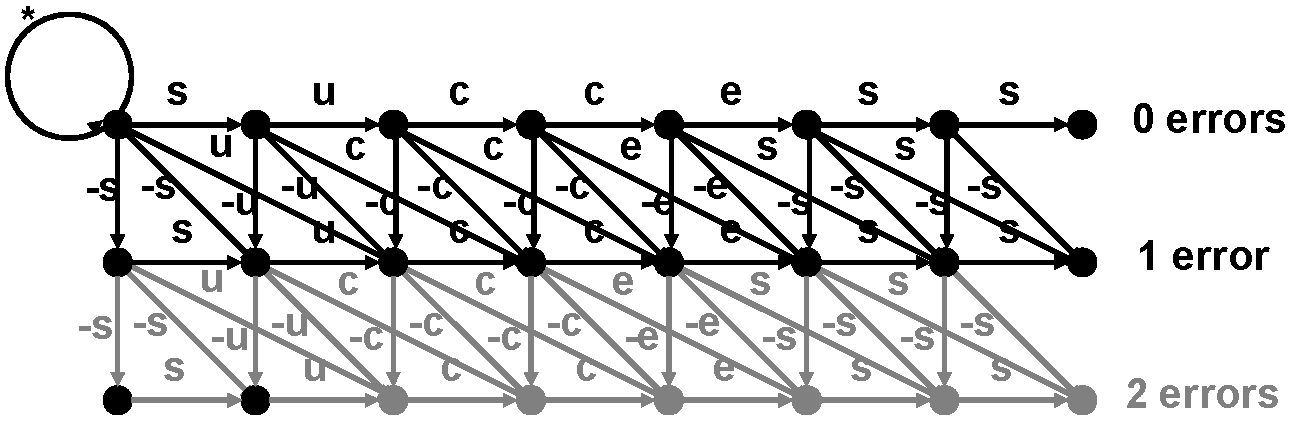
\includegraphics[scale=0.65]{./figures/levensthein.pdf}
\end{center}

\caption{An example of the Levensthein transducer for the word \emph{"success"}. (Taken from the study material for the \emph{Information Retrieval Systems} course at MFF UK by Michal Kopecký.)}
\end{figure}

For bigger databases the online algorithms begin to be very slow a preprocessing of the database is necessary. Some sophisticated indexing methods are used, among them the suffix trees or $n$-gram indexes. The candidates retrieved from such indexes are later examined more carefully.

\subsection{Current TM tools}

The tool most frequently used by the professional translator is \emph{SDL Trados}. It was originally developed by the German company Trados which was later acquired by its biggest rival, British SDL. It became popular mostly because of its integration to Microsoft Office starting in middle nighties. It is a very complex software. Except the actual tool for the end users, it includes central servers where a translation agency can gather its data and from where the data can be distributed to the translators' PCs and sophisticated tools for team work. The other popular translation memories are DeJaVu by the French company Atril or Wordfast by an American company of the same name. According to a 2006 survey\footnote{Elina Lagoudaki: Translation Memories Survey 2006: 
Users' perceptions around TM use. In: \emph{[Translating and the Computer 2006.} London: Aslib, 2006.} 54 \% of profession translator world wide used products by Trados or SDL, 17 \% Wordfast and 16 \% Deja Vu.

There are also few open source translation memories projects, mostly not really elaborated and with a small community. IBM has recently released its internally used software under the Eclipse Public Licence. A widely used open source tool is called OmegaT. Is is a cross-platform software which provides very complex functionality. It can be interconnected with the Trados servers, supports most of the translation memory formats and supports also a lot of textual formats, but without integration to other software. It is also commonly used for translation of open source software. According to previously mentioned survey it is used by only 3 \% of professional translators.

\begin{figure}
\begin{center}
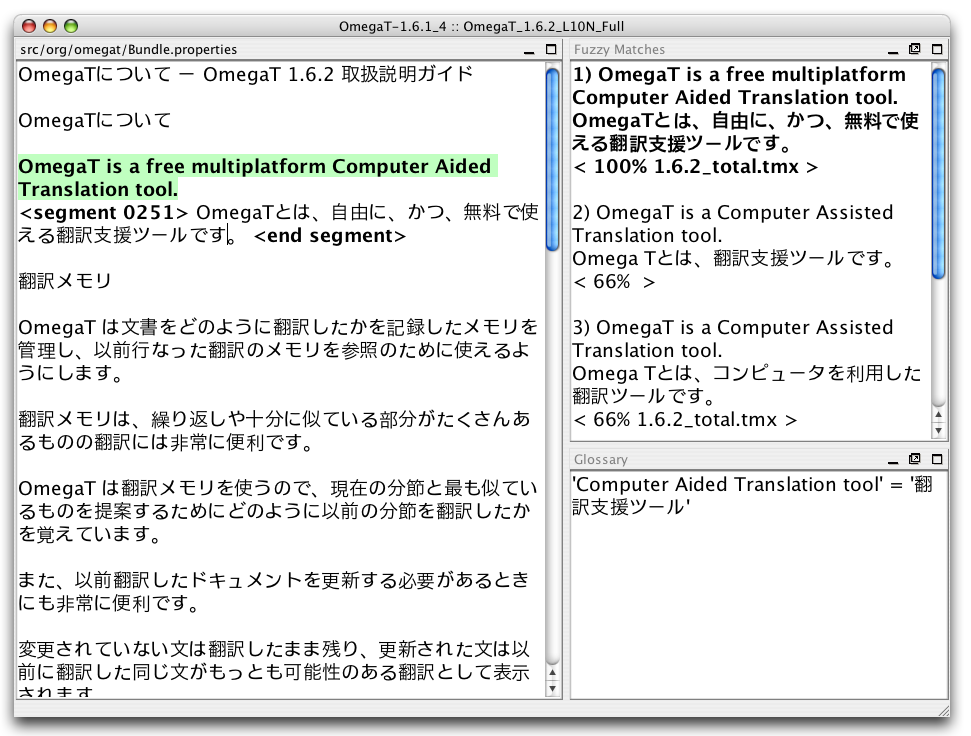
\includegraphics[scale=.4]{./figures/omegat.png}
\end{center}

\caption{A screenshot of the OmegaT version 1.6}

\end{figure}

There is also a translation memory project which is somehow similar to our project. It is called \emph{MyMemory} and it was created by a Italian translation agency Translated.net. It is a big general purpose translation memory available as a remote service via the Internet. It contains translation from various domains which can be used either separately or altogether. Using of the MyMemory is free of charge under condition the translations produced using the service will be provided as a data to the service.